\documentclass[12pt,twoside,letterpaper]{article}
\usepackage{graphicx}
\setlength\topmargin{0in}
\setlength\headheight{0in}
\setlength\headsep{0in}
\setlength\textheight{9.0in}
\setlength\textwidth{6.5in}
\setlength\oddsidemargin{0in}
\setlength\evensidemargin{0in}
\setlength{\parskip}{12pt}
\pagestyle{plain}
\raggedright
\title{Thread-Level Parallelism Available in Imperative Programs Dissertation Proposal}
\author{Cameron Lowell Palmer}
\date{Fall 2008}
\begin{document}
\maketitle
The age of the multi-processor desktop computer has been with us for a few years now. As we have run out of ways to ramp up processor clock, companies have put multiple processors on a die to increase performance. For the typical desktop running a handful of applications and an operating system, this direction has improved real-world performance for users considerably. Of course, this improvement in performance does not come from a proliferation of multi-threaded programming or a magical compiler technique; it relies simply on the ability of the operating system to interleave the programs' execution on your two or more processors. Applications largely remain single-threaded, unable to take advantage of the multi-threading on their own. To take advantage of larger numbers of processors, we will need to extract more parallelism from imperative programs.

The limits of instruction-level parallelism (ILP) have been investigated in \cite{Tjaden:1970p214} and later in \cite{Wall:1991p191}. \cite{Tjaden:1970p214} found very little ILP within basic blocks, the code between conditional branches. That study seemed flawed because more parallelism was being discovered in practice in part because they were looking beyond basic block boundaries. \cite{Wall:1991p191} attempted a very aggressive ILP discovery eliminating all barriers to maximum parallelism, and still little parallelism was found. A different way of finding parallelism through VLIW was discussed in \cite{Nicolau:1984p217} and yielded a much different result. \cite{Lam:1992p188} built on the \cite{Wall:1991p191} paper and investigated the limiting factors in instruction-level parallelism. They found control flow to be the root cause and suggested some ways of combating control flow through techniques like speculative execution. Later this previous work was summarized by \cite{Rau:1992p211}. I propose to build on this body of work and investigate the limits of thread-level parallelism (TLP) in imperative code. I want to look at TLP because it is better suited to multi-core processors, and potentially compiler techniques for automatically parallelizing code. First, performing a limit study of TLP will give us an upper bound on the amount of parallelism we can extract from existing programs in the SPEC CPU benchmark suite, and then map to the multi-core processors available on most desktops. From this point, we can investigate different code motion techniques or methods of extracting parallelism, different architectures, and hopefully realize the potential of modern multi-core processors. In summary, this research will quantify how much TLP is available in imperative code.

\section*{Background Information}
\subsection*{Basic Processor Technology}
The modern processor, or von Neumann architecture, is broken into several distinct stages. These stages within the context of the MIPS processor are Instruction Fetch (IF), Instruction Decode (ID), Execute (EX), Memory Access (MA), and Write Back (WB). An instruction is taken from the queue of instructions to be executed, decoded and the program counter (PC) incremented, executed through a manipulation in the Arithmetic Logic Unit (ALU), possibly transfer to or from main memory, and finally write results into a register. The ALU is one of the components that make up every CPU, and these components that perform the work of the stages are referred to as functional units. In this simplistic version of computer processor architecture, every instruction completes in one-cycle and the cycle is the length of time required to complete the longest instruction. 

The next logical step is to use these stage boundaries to divide up instructions into multiple cycles by pipelining the processor. At any given stage, the processor can be using all of the functional units in the processor simultaneously. For example, one instruction could be decoding while a second instruction could be in the execute phase, and a third in write back. This system allows instructions to be completed every cycle in the case where there are no dependences between instructions. An illustration of the simple pipelined architecture can be found in Figure \ref{mips_pipeline}.

We can further subdivide the stages of the processor, resulting in a superpipelined architecture. If we add multiple sets of parallel functional units within the processor and allow our processor to issue multiple instructions simultaneously, we call this superscalar. The PowerPC 970 processor is an example of a superscalar design that has four ALUs, two Floating Point Units (FPUs), and two Single Instruction Mulitple Data (SIMD) units. The combination of superscalar and superpipelining can get the processor to complete multiple instructions per cycle.

Realistically, the instructions are not going to be dependence-free, and they may not be in an ideal order, resulting in stalls where nothing is happening in a particular part of the processor for several cycles. Therefore, we need instruction reordering to help hide latencies and keep the functional units busy. Instruction reordering has been in computing hardware since the CDC 6600 (Scoreboarding) and the IBM System 360 Model 91 (Tomasulo's Algorithm). This allows the processor to reorder instructions on-the-fly to maximize the throughput of instructions and hopefully get us close to one instruction completing per cycle. Instruction reordering can also be done by the compiler, and in architectures like VLIW, this compile-time instruction ordering is critical.

\begin{figure}
	\begin{center}
		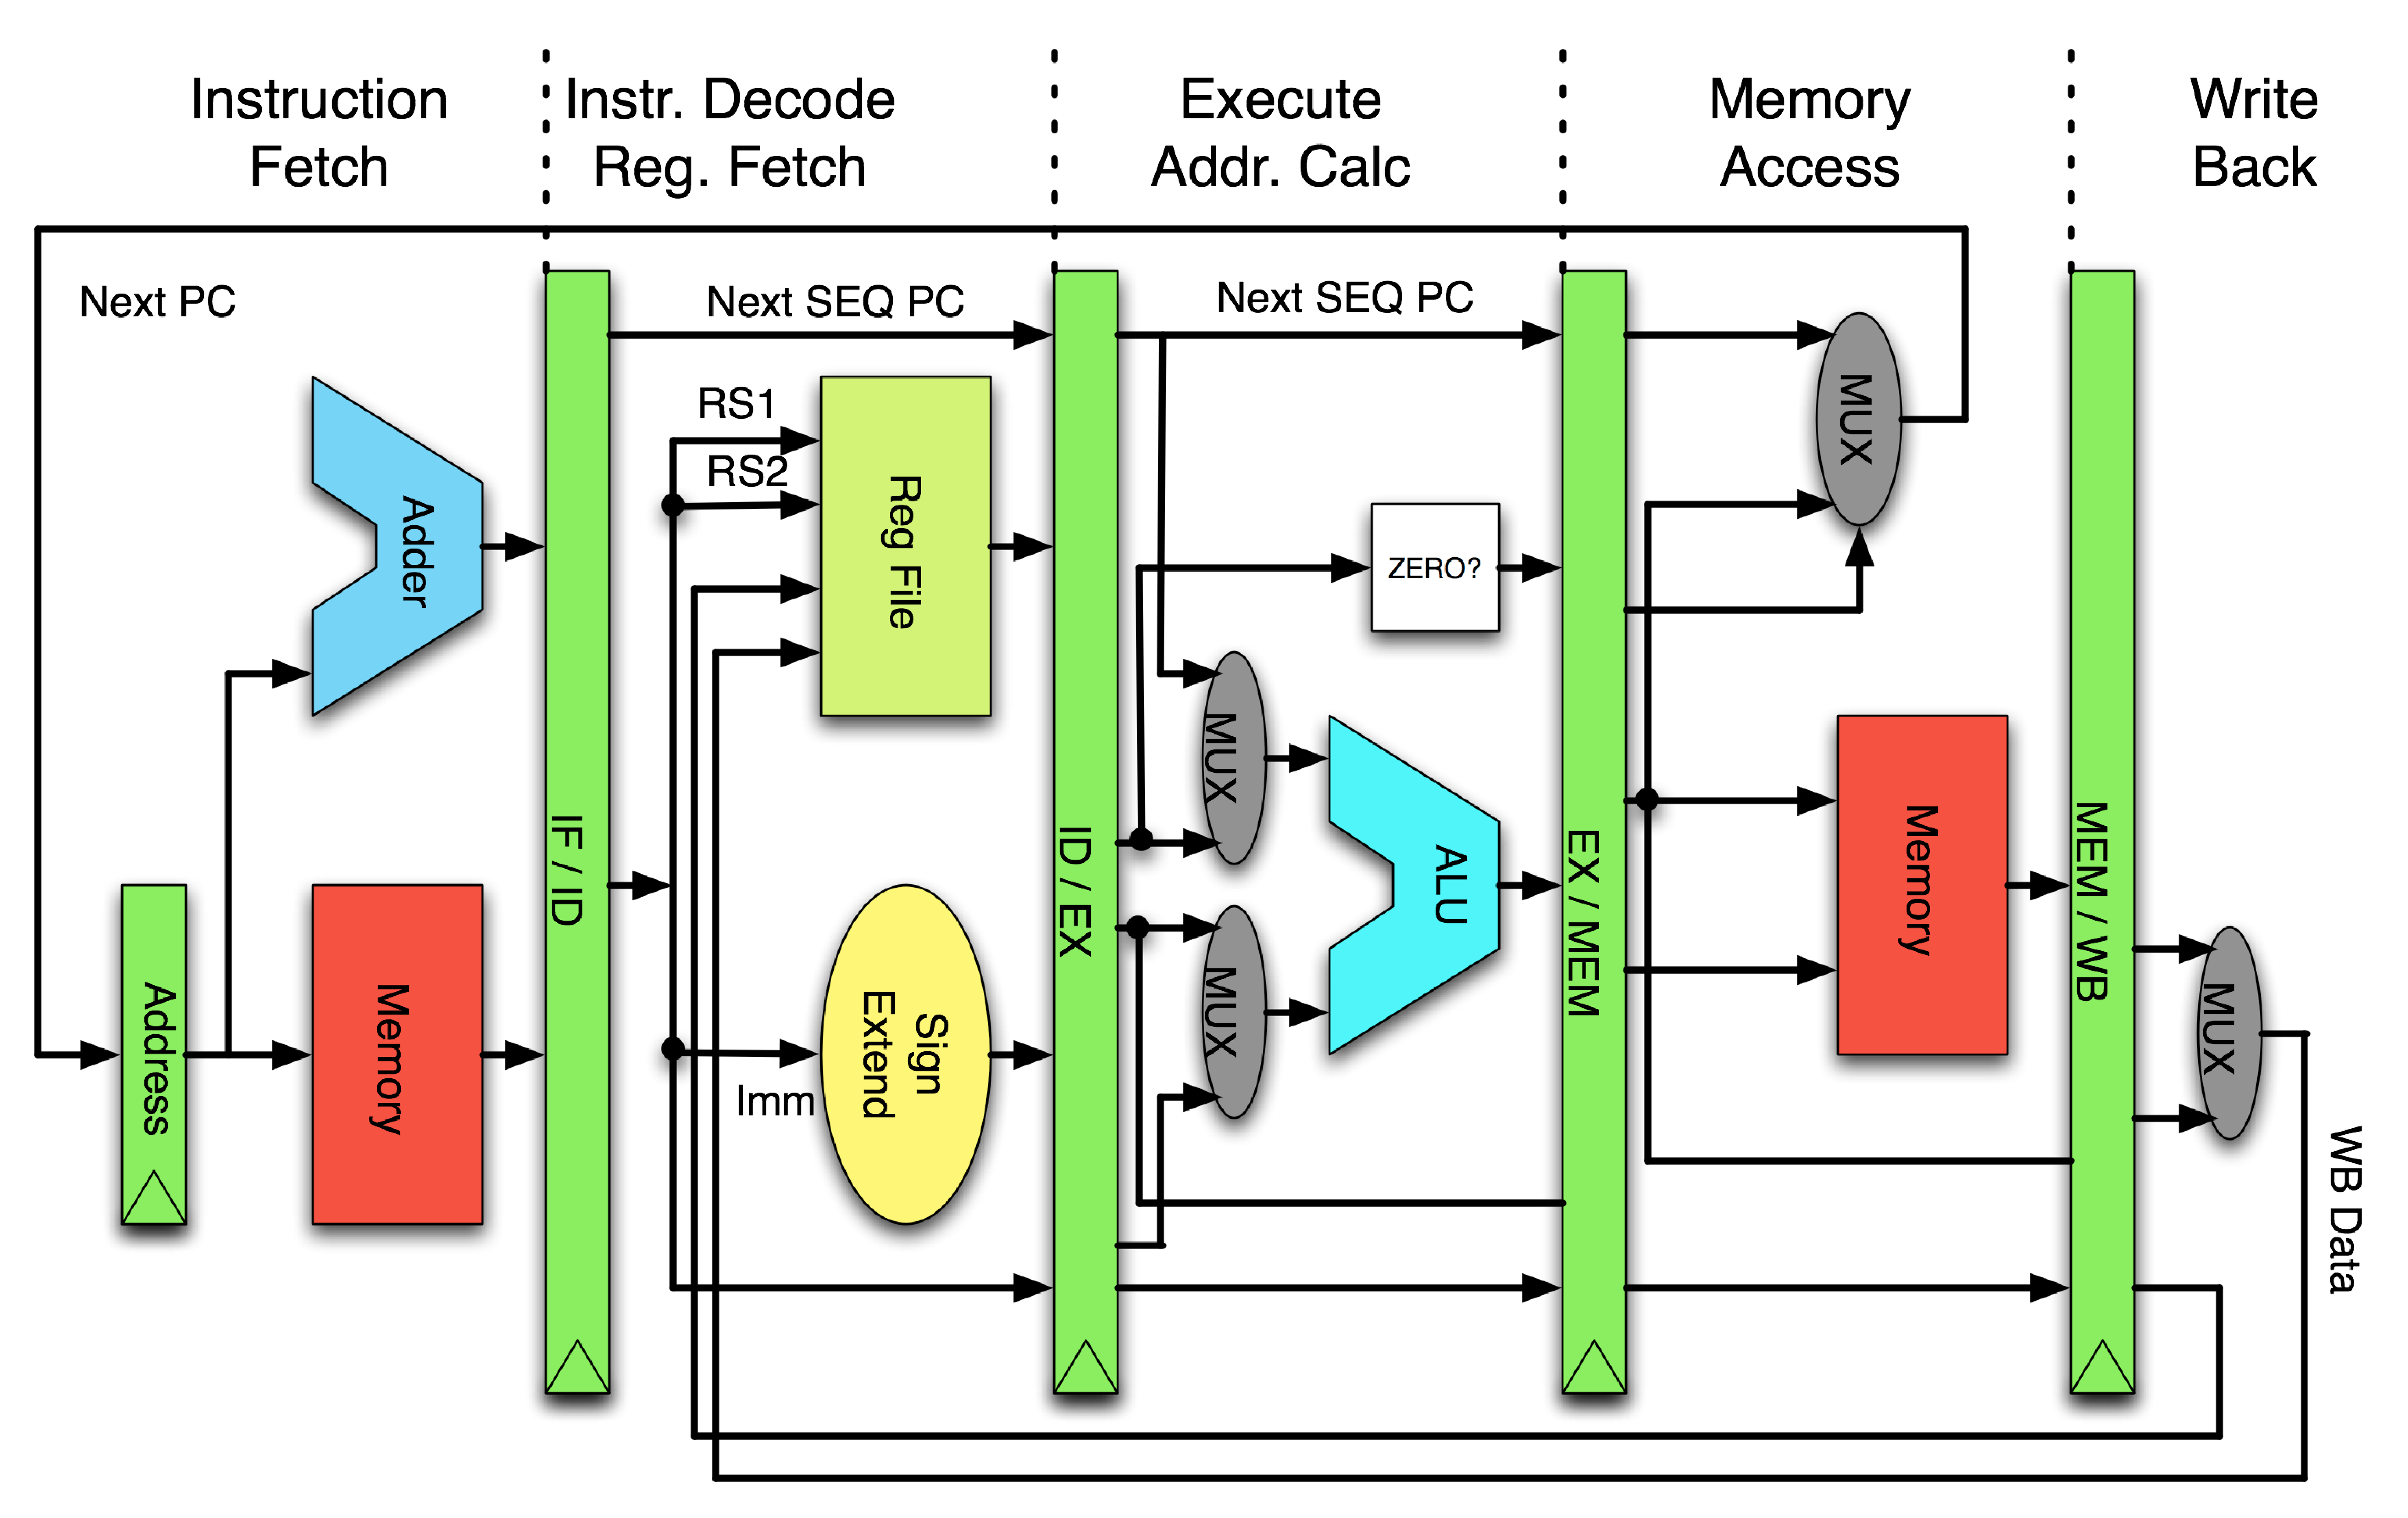
\includegraphics[angle=-90,scale=.65]{Pipeline_MIPS.epsi}
	\end{center}
	
	\caption{A simple pipelined processor}
	\label{mips_pipeline}
\end{figure}

\subsection*{Memory}
The processor will need memory, and the most common method of interfacing memory and the processor is through some sort of cache. The speed of memory has not kept pace with processor speed increases, so cache helps hide the slow speed of main memory.  

\begin{quote}
Although CPUs are a thousand times faster, memory speed has increased only by a factor of ten or so. Back in the 1980s, reading a bit from main memory took a few hundred nanoseconds, which was also the time needed to execute a single instruction in a CPU. The memory and the processor cycles were well matched. Today, a processor could execute a hundred instructions in the time it takes to get data from memory. - \cite{Hayes:2007p4}
\end{quote}

We have therefore developed very good cache predictors to try and have the correct instructions or data in cache to avoid the significant delay. Of course, cache introduces its own problems, energy consumption, and lack of predictable latency which makes cache less useful in real-time embedded designs. Cache memory uses a significant amount of space on the CPU die and has caused some processors like Cell to eliminate cache altogether, or explore new approaches, such as scratchpad memory.

\subsection*{Diminishing Returns}
I took note of the change in processor design when the Pentium 4 reached 3.0GHz and Intel added a new feature called hyper-threading (HT) or simultaneous multi-threading (SMT) to the untrademarked, the idea being that the they could keep the functional units of the processor busy if a single processor appeared as two processors to the operating system. Actually, if the operating system (OS) did not treat the processor as logical vs. physical processors, they could negatively impact performance; however, in general, the OS need not do much to take advantage of this technology. Hyper-threading was for many the harbinger of the move to multi-core processing. It was at this moment that I began to wonder why HT is necessary, and why not just attain the necessary performance by going to 6.0Ghz? Why have new processors actually seemingly slowed down? For example, the current Intel Core2 processors dropped down to $\sim$2.4GHz.

The doubling of transistors that can fit on a die every 18 months, combined with smaller transistors, has had the nice advantage of packing more transistors into the same die space. In general, the amount of dynamic power consumption grows exponentially with die size. However, with technology like clock gating, they have limited the growth of dynamic power consumption to nearly linear. Real-world processors have grown by about .7 in die size and dynamic power consumption has grown by about .85. 

Leakage, or non-useful power consumption, is occuring through the circuit when the circuit should be closed (sub-threshold leakage), and in general through the insulator (gate oxide tunnelling). This leakage is caused by shrinking the transistor size, and increasing switching frequency. Leakage power increases exponentially as die size decreases, and has provided a challenge to further shrinking die size or packing more transistors into the die space because it is not as easily controlled as dynamic switching power. In a news article from AnandTech, it was said a Pentium 4, according to Intel, if built with a 45nm process, would leak about 100W. This leakage, even if acceptable, would have to be dissipated in the form of heat, and would certainly require some elaborate cooling mechanism.

There are strategies to coping with leakage, but, in the end, leakage, wire delay, and other issues conspire to make complex, deeply pipelined processors problematic. Intel, AMD, IBM have begun to alter their strategies and started putting multiple CPUs on the die to sidestep the issue of increasing processor frequency.

\subsection*{Multi-core processors to the rescue, or ... we have multiple cores, now what?}
With the industry moving to multi-core processors, we have gained in real-world performance by simply taking advantage of the operating systems' ability to interleave application execution on multiple processors. Brilliant, just like ILP in processors, no programming changes to existing applications are necessary to get a performance boost.

The story does not end here because we are still typically talking about only two to four processors in a desktop class machine. As we see eight, sixteen, or higher numbers of processors become more prevalent will we continue to take advantage of the potential of these machines?

To take advantage of these machines, we will need to generate multi-threaded programs that can execute on as many processors as possible. These threads are generated by programmers identifying parallelism in their code, and then using any of the number of thread models to encapsulate sections of their code. There are limited general compiler techniques for thread-level code generation, and that leaves the work to programmers.

As we know, writing thread-safe code is hard and time consuming to do. Even expert programmers have trouble writing threads, and still only apply it to small portions of their code base. That is why we need to explore automatic parallelization of code through the compiler if we hope to take advantage of this new processor architecture.

\section*{Limited parallelism}
ILP is the amount of parallelism that can be found in instructions through reordering. The first commercial machines that could exploit ILP were CDC’s 6600 and IBM’s System 360 Model 91, both in the 1960s, using Scoreboarding and Tomasulo’s Algorithm respectively. Today the idea of multiple issue and out-of-order execution is found in most processors on the market, and is the cornerstone of superscalar, superpipelined desktop processors on the market today. To make processors perform faster we want to finish instructions every cycle, and to do that we must issue multiple instructions each cycle as operands become available, and keep all the functional units as busy as possible.

One of the best attempts at determining the amount of ILP available in the average program was attempted by David Wall in \cite{Wall:1991p191}. Joseph Fisher said of Wall's paper \cite{Rau:1992p211} that it is possible that a new technique could discover more parallelism than Wall does in this paper, just like more ILP was available in 1993 than the pessimistic 1.86 found in basic blocks in \cite{Tjaden:1970p214}, but this paper does the best job of performing an aggressive limit study of ILP.

Wall identifies early in the paper what limits parallelism. One problem is dependencies between instructions. True dependencies, where the outcome of one instruction feeds into the next instruction, cannot be removed. The true dependence represents the fundamental ordering inherent in tasks, just like I must obtain food before consuming it. Other tasks are not as rigidly ordered, but an artificial register dependency can be created because of poor planning during register assignment. This poor planning might be the reuse of a register that prevents an independent task from executing in parallel and can be addressed with register renaming. A similar but more difficult version of this problem can happen with memory operations. It can be difficult to determine at compile time if two operations are using the same memory location. To use Wall's example:

\begin{quote}
r1 := 0[r9] \\
4[r16] := r3
\end{quote}

We cannot tell if this load and store is to the same location or different locations. We must use alias analysis to try to clear this up, but in practice we often err on the side of safety and enforce strict ordering.

Wall, unlike early investigators of ILP, looked beyond basic blocks. The number of instructions Wall found between jumps (a basic block) is small, often averaging less than 6. According to \cite{Hennessy:2003p277}, MIPS has between 3-6 instructions in its basic blocks as another example. These small basic blocks require us to stop and wait for the branch evaluation to occur so that we can choose the right path. In order to hide these latencies, we can use branch prediction and potentially speculation. This introduces the problem of speculative fanout, since jumps are so frequent that you can still be evaluating a previous branch when you encounter the next. Loop unrolling is another way to enlarge basic blocks to get more parallelism. When we unroll a loop numerous times, we remove branches and have more instructions to move. Wall also mentions software pipelining, and trace scheduling to further enlarge blocks. The speedups for non-numeric programs ranged between 4.1 and 7.4, which is disappointing considering the assumptions.

Building on Wall's work in \cite{Lam:1992p188} the authors try to increase parallelism by first assuming the limitation is control-flow. Their interpretation of the Wall data is that control-flow limits parallelism for non-numeric programs to 4.1 to 7.4. This assumption also agrees with the findings of \cite{Riseman:1972p215} which found 51x speedup without control-flow, and \cite{Nicolau:1984p217}. All three papers discuss the oracle machine model that makes perfect branch predictions, and each time the elimination of control-flow unlocks significant parallelism in the code.

\section*{Overcoming control-flow}
A commonly discussed solution for the limitations of control-flow is to speculatively execute branches, only stopping to resolve mispredicted branches. I propose we try to establish a limit to the parallelism available at the thread-level, accounting for different models and speculation. If we can establish an upper-bound on speculatively executed threads across multiple processors we can establish the speedups achievable from our new processor architectural direction.

\section*{Experimental Methodology}
The SPEC CPU benchmarks are designed to test CPU, Memory, and Compiler performance, and are designed to exercise only these components of the system. This would be a sufficient measure of performance if this proposal were limited to a 'real-world' compilers and computer systems. However, we would like this to be a limit study of thread-level parallelism, not a particular architecture. Therefore, to meet this requirement, we will use a simulator to relax our constraints as in the Wall paper.

We will assume unlimited computing resources like registers and memory, make all instructions take one cycle, and assume perfect memory disambiguation. This will leave us with only the control-flow constraints imposed by the natural ordering of instructions created by true dependences, and conditional branches.

Using GCC and the SPEC CPU benchmarks as a basis for our compiler work, we can add code to manipulate GCC's static-single assignment (SSA) form to identify potential threads. This thread identification could simply be turning every basic block into a thread, looking at Phi nodes as a thread boundary, or examine program slicing methods to generate threads.

\section*{Milestones}
\begin{enumerate}
\item Identify a simulator, or build a simulator that can accept the binaries generated by the Integer portion of SPEC CPU2006 benchmarks using GCC 4.x as our compiler. It also needs to be capable of allowing multiple threads of execution, manipulate instruction cycle count, and calculate the performance of the threaded application.
\item Add appropriate code to the GCC C/C++ compiler to allow different threading strategies:
    \begin{itemize}
		\item loop-level
		\item basic-block
		\item function-level
		\item global (more than one block, but less than a function possibly after removing some control flow through predicated execution)
    \end{itemize}
\item Run the SPEC CPU2006 Integer benchmarks with the different threading strategies and measure performance.
\end{enumerate}
\bibliographystyle{apalike}
\bibliography{tlp_limits}
\end{document}
